\documentclass[12pt,letterpaper]{article}
\usepackage[margin=1.75in]{geometry}
\usepackage[english]{babel}
\usepackage[utf8x]{inputenc}
\usepackage{amsmath}
\usepackage{amssymb} 
\usepackage{amsthm}
\usepackage[retainorgcmds]{IEEEtrantools}
\usepackage{graphicx}
\usepackage{tabularx}
\usepackage{subfig}
\usepackage{kpfonts}    % for nice fonts
\usepackage{microtype} 
\usepackage{booktabs}   % for nice tables
\usepackage{bm}         % for bold math
\usepackage{listings}   % for inserting code
\usepackage{verbatim}   % useful for program listings
\usepackage{color}  
\usepackage[colorlinks=false]{hyperref}   % use for hypertext
\usepackage[colorinlistoftodos]{todonotes}
\usepackage{natbib}
\usepackage{indentfirst}
\usepackage{csquotes}
\usepackage{hyperref}


\theoremstyle{definition}   % the choice of the theorem block style
\newtheorem*{remark}{Remark}    % the remark do not have number index



\setlength {\marginparwidth }{2cm}    % I don't know what does it mean, I just add this line to avoid the annoying suggestion

\begin{document}

%+Title
\title{\textbf{Notes on \cite{kamenica2019bayesian}}\\{\small \textbf{Bayesian Persuasion and Information Design}}}
\author{Quan Li}
\date{\today}
\maketitle
%-Title

%+Abstract
\begin{abstract}
This article review the literature that answers the questions of what is the optimal information that should be revealed.\footnote{For instance,	``\textit{A school may improve its students’ job outcomes if it issues only coarse grades. Google can reduce congestion on roads by giving drivers noisy information about the state of traffic. A social planner might raise everyone’s welfare by providing only partial information about solvency of banks. All of this can happen even when everyone is \textbf{fully rational} and \textbf{understands the data-generating process}.}"} 
\end{abstract}
%-Abstract


\section{What is Bayesian Persuasion?}



  
Economic behavior may be driven by three factors:
\begin{itemize}
	\item Preference
	\item Technology
	\item Information
\end{itemize}

Consequently, there are three broad ways of influencing economic outcomes:\footnote{These methods are not necessarily isolated, \cite{li2017model} add transfers to the persuasion model, \cite{lewis1994supplying} study a monopolist who chooses both what price to charge and what information to provide to consumers about their valuations for the firm's product.}

\begin{itemize}
	\item Change the (induced) preference over actions via incentives
	\begin{itemize}
		\item contingent payments
		\item threat of violence
		\item supply of complementary goods
	\end{itemize}
	\item Technology: make it easier for a decision maker to achieve it\footnote{The methods used in nudging and choice structure \citep{thalernudge} can be seen as technological interventions, as argued by \cite{kamenica2012behavioral}. For instance, teaching the taxi drivers to open the car door with their right hand in order to reduce the chance that they cause an accident can be regarded as a technological innovation.}
	\item \textbf{Persuasion: influencing behavior via provision of information \citep{kamenica2011bayesian}}
\end{itemize}

\emph{Bayesian Persuasion}: \textbf{Bayesian} means the decision maker is standard, i.e. she understands how information is generated and react to information in a rational (\textbf{Bayesian}) manner.\footnote{It is also referred to as \emph{Information Design}, but the former is probably used more when the designer is one of the player and there is a single receiver, while the latter is used more when the designer is a social planner or there are multiple receivers.} 

\subsubsection*{The comparison between \emph{Information Design} and \emph{Mechanism Design} \citep*{bergemann2016bayesb, taneva2019information}}

\begin{itemize}
	\item \textbf{Mechanism Design}: the allocation of information (i.e., who knows what) is given, the designer select the game that the agents will play to influence the outcome.
	\item \textbf{Information Design}: the game is given, the designer influences the outcome by specifying the allocation of information. 
\end{itemize}

\subsubsection*{Bayesian Persuasion is a communication protocol}

Before, we have models of communication: 
\begin{itemize}
	\item Cheap talk \citep{crawford1982strategic}
	\item Verifiable message \citep{grossman1981informational,milgrom1981good}
	\item Signaling game \citep{spence1978job}
\end{itemize}

\subsubsection*{The full commitment formulation of Bayesian Persuasion}

Relative the above models, Bayesian Persuasion endows the sender with more commitment power. It allows the sender to commit to sending any distribution of messages as a function of the state of the world. \footnote{\cite{min2020bayesian} relax the assumption, study the results under \emph{partial commitment}}

The equivalence between the alternative models and Bayesian persuasion (??) \citep{gentzkow2017disclosure}

\subsection*{Other surveys of Information Design}

This review exclusively focus on the desire of the sender to influence.

\cite{bergemann2019markets} studies the markets where a seller design information to sell it. \footnote{For example, \cite{bergemann2018design} and \cite{kastl2018selling}}

\subsubsection*{The relationship with Bayes correlated equilibria \citep{bergemann2013robust}}

Bayes correlated equilibria take as given a basic game: 
\begin{itemize}
	\item a set of players
	\item a set of feasible actions for each player
	\item players' payoffs as a function of the state of the world and the actions taken
\end{itemize}

\emph{Describe the set of all possible outcomes that could arise (as Bayes Nash equilibria) \textbf{regardless of what each player knows(about the state and the other player know)}}


It predicts the outcome of the basic game that is robust to the uncertainty about the knowledge, and by definition, it coincides the outcome can be attained through information design.

\begin{center}
	A Bayesian persuasion problem

\[\Updownarrow\]

A problem of selecting an optimal \emph{Bayes correlated equilibrium} given an objective function 

\end{center}


\subsubsection*{More applied strand}
Include the following interesting papers:
\begin{itemize}
	\item Financial stress tests \citep{goldstein2018stress}
	\item Grading in schools \citep{ostrovsky2010information}
	\item Matching platforms \citep{romanyuk2019cream}
	\item Price discrimination \citep{bergemann2015limits}
\end{itemize}


\section{The Model and its Interpretations}

\subsection{The Basic Model}

\subsubsection*{The specification:}
\begin{itemize}
	\item Agents: \{Sender, Receiver\}
	\item Action: $a \in A$
	\item State: $\omega \in \Omega$ 
	\item Utility: 
	\begin{itemize}
		\item Sender: $v(a, \omega)$\footnote{We may be willing to view $v$ as the \emph{welfare function} if we regard the sender as a social designer.}
		\item Receiver: $u(a, \omega)$
	\end{itemize}
	\item Belief: common prior $\mu_0 \in \Delta \Omega$
\end{itemize}

\subsubsection*{The key object: \emph{Signal} \footnote{It goes by many other names, including signal structure, information structure, experiment, Black-well experiment, data-generating process} }
\begin{itemize}
	\item Signal realizations: $S$\footnote{it suffices to assume $|S| \geq min\{|A|, |\Omega|\}$, (??) \emph{Is there some economic consider relevant to care about the cardinality of $S$?}}
	\item Signal: $\pi  : \Omega \rightarrow \Delta (S)\footnote{It takes form like $P(s | \omega)$} \Leftrightarrow\footnote{For $P(s | \omega) = \frac{P(s, \omega)}{\mu_{0}(\omega)}$, and $\mu_{0}$ is given at the very beginning} \Delta (\Omega \times S) \in \Pi$ 
\end{itemize}

\subsubsection*{Timing}
\begin{enumerate}
	\item Sender chooses a signal $\pi$
	\item Receiver observes which signal was chosen
	\item $\omega$ is realized by $\mu_0$
	\item $s$ is realized according to $\pi(\omega)$\footnote{Remember $\pi(\omega) \in \Delta (S)$ }
	\item Receiver observes the realized $s$
	\item Receiver takes action $a$
\end{enumerate}

\subsubsection*{The receiver's mechanical behavior}
\begin{itemize}
	\item Bayesian Updating:
	\[\mu_{\pi}(\omega | s) = \frac{\pi(s | \omega) \mu_0(\omega)}{\sum_{\omega'} \pi(s | \omega') \mu(\omega')}\]
	\item Optimization\footnote{The receiver's strategy is a mapping from $\Pi$ to the mapping from the set of signal realizations $S$ to the set of actions $A$}:
	\[a^*(\mu_{\pi}(\cdot | s)) \in argmax_{a \in A} \mathbb{E}_{\omega \sim \mu_{\pi}(\cdot | s)} u(a, \omega) \]
\end{itemize}

\subsubsection*{The sender's backward induction problem}

\begin{equation}
	\label{Equation 1}
	\pi^* \in argmax_{\pi \in \Pi} \mathbb{E}_{\omega \sim \mu_{0}} \mathbb{E}_{s \sim \pi(\omega)} v\left(a^{*}\left(\mu_{\pi}(\cdot \mid s)\right), \omega\right)
\end{equation}


\subsubsection*{What should we care about?}

The model is quite general, it may be daunting or meaningless to find out a general optimal signal. 
So we are willing to recasting the problem to make it more precise and more approachable.(See Section 3)

\vspace{0.5cm}

For the following several reasons:
\begin{itemize}
	\item $\Pi$ is a pretty large set
	\item The choice of $\pi$ influences the sender's payoff both by changing the second expectation ($\mathbb{E}_{s \sim \pi(\omega)}$) and by the optimal action $a^{*}\left(\mu_{\pi}(\cdot \mid s)\right)$ chosen by the receiver
\end{itemize}

\subsection{Interpretations}

\subsubsection*{The courtroom example}

\begin{itemize}
	\item Agents: \textbf{\{prosecutor, judge\}}
	\item Action: \textbf{convict or not}
	\item State: \textbf{the guilt of the defendant}
	\item Utility:
	      \begin{itemize}
			  \item Prosecutor: \textbf{always prefers conviction}
			  \item Judge: \textbf{match the truth}
		  \end{itemize}
	\item Signal: \textbf{\{forensic tests, questions asked to witnesses\}}\footnote{If the assumption of finding out the whole truth is implausible, we can redefine the state as the realizations of the most informative signal.}
\end{itemize}


\subsubsection*{Grades in schools(??\footnote{There are some tricky details I cannot understand, for example, the author assume schools know the ability (true state) before choosing the grading policy.})}

\begin{itemize}
	\item Agents: \textbf{\{school, the labor market\}}
	\item Action: \textbf{placement of the student}
	\item State: \textbf{the ability of the student}
	\item Utility:
	      \begin{itemize}
			  \item school: ague by yourself
			  \item the labor market: think about it by yourself
		  \end{itemize}
	\item Signal: \textbf{the school's grading policy} 
\end{itemize}

It maybe combined with the job market matching model \citep{chen2020learning} and delegation model \citep{frankel2014aligned} to study a model with grading policy and job market.

\subsubsection*{Speeding of drivers \citep*{lazear2006speeding}}

Original model:
\begin{itemize}
	\item $Z$ miles of road
	\item A driver choose to speed or not on each mile
	\item Speeding utility $V \leq K$ Fine for Speeding
	\item There $G \leq Z$ police, and each can patrol one mile of road 
	\item The police wish to minimize the number of miles over which drivers speed.
\end{itemize}
It is equivalent to the following Bayesian persuasion model:
\begin{itemize}
	\item Agents: \textbf{\{the police, the driver\}}
	\item Action: \textbf{speed or not}
	\item State: \textbf{the presence of a policeman on a given mile}
	\item Utility:
	      \begin{itemize}
			  \item 
			  \item 
		  \end{itemize}
	\item Common belief: $\mu_0 = G/Z$
	\item Signal: \textbf{the predictability of the patrolling strategy} 
\end{itemize}

Typical signals:
\begin{itemize}
	\item Randomly set up the speed traps $\Rightarrow$ uninformative signal $\underline{\pi}$ $\Rightarrow$ $\mu_{\underline{\pi}}( \cdot | s) = G/Z$
	\item Always patrol the exact same locations $\Rightarrow$ fully informative signal $\overline{\pi}$ $\Rightarrow$ $\mu_{\overline{\pi}}( \cdot | s) = 0\text{ or }1$
\end{itemize}

Other applications involve yet other interpretations of how a signal is generated \citep*{best2020persuasion}.


\subsubsection*{The justification of commitment assumption}

It varies substantially across applications.







\section{Sender's Optimization Problem}

\subsection{Concavification}

From the sender's view, what matters is the \emph{posterior beliefs}, not the signals. So we reformulate the problem as follows:

An important observation\footnote{$\mathbb{E}_s$ means take expectation with respect to $s$, that is, use the probability of appearance of $s$ to calculate the expectation}

\[\mathbb{E}_s  \mu(\omega \mid s) = \mu_0 (\omega)\]


If we use a rather formal notation 
$\tau = <\pi>$ to indicate that a distribution of posterior $\mu$ induced by $\pi$ 
\footnote{Algebraically, 
a signal induces a distribution of posterior 
$\tau$ if $\tau(\mu) = \sum_{s:\mu_{\pi(\cdot|s)} = \mu} \sum_{\omega' \in \Omega} \pi(s | \omega') \mu_0(\omega')$}


The equation transforms to 

\[\mathbb{E}_{\mu \sim \tau}  \mu = \mu_0\]

And for the expectation is commutative, then we can reformulate the sender's expected utility (1) as:
\[max_{\pi \in \Pi} \mathbb{E}_{\omega \sim \mu_{0}} \mathbb{E}_{s \sim \pi(\omega)} v\left(a^{*}\left(\mu_{\pi}(\cdot \mid s)\right), \omega\right)\]

\begin{equation}
	= \max_{\tau} \mathbb{E}_{\mu \sim \tau} \hat{v}(\mu) 
\end{equation}

s.t. $\mathbb{E}_{\mu \sim \tau}  \mu = \mu_0$, where as $\hat{v}(\mu) = \mathbb{E}_{\omega \sim \mu} v(a^*(\mu), \omega)$

\subsubsection*{A nice geometric interpretation}

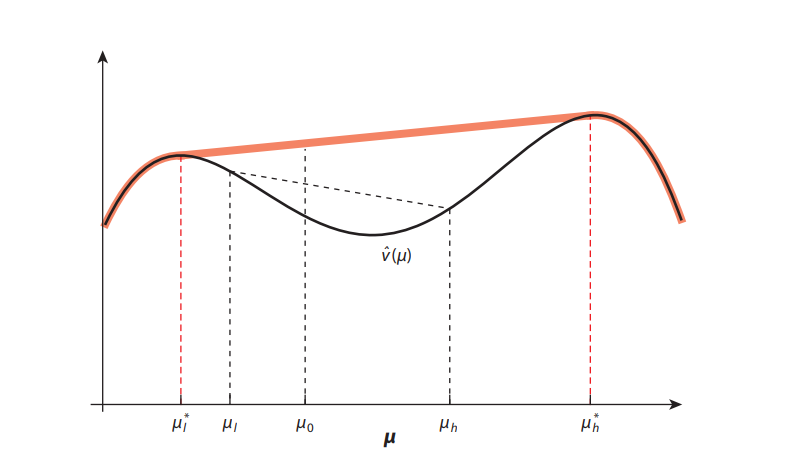
\includegraphics[scale=0.6]{concavification.png}

\begin{itemize}
	\item The concavification of $\hat{v}$ evaluated at $\mu_0$ equals $max\{z \mid (\mu_0, z) \in co(\hat{v})\}$\footnote{$co(\hat{v})$ denotes the convex hull of the graph of $\hat{v}$}
	\item Send's utility under the optimal signal is precisely the concavification of $\hat{v}$ evaluated at $\mu_o$
\end{itemize}

\begin{remark}
	If there is more than three states, we cannot plot $\hat{v}$ anymore, but the concavification approach can still be used to derive some qualitative features of the optimal signal(see \autoref{Section 4}).
\end{remark}

\subsubsection*{The intellectual history of concavification approach}

Characterizing the equilibria of the following repeated games of incomplete information is analogous to the \autoref{Equation 1} \citep{aumann1966game}
\begin{itemize}
	\item Two players: {Informed player($I$), Uninformed player($U$)}
	\item Two \emph{zero-sum} games: $G_A$ and $G_B$
	\item Identical action spaces
	\item With $\mu_0$, the players will repeatedly play $G_A$ ad infinitum, and $G_B$ otherwise.
	\item Before each period, $I$ knows which game they will be playing
	\item After each period, $U$ observes the action of $I$, but she does not observe her payoff, nor which game they had played
	\item Each player seek to maximize their undiscounted average payoff (??\footnote{Why is it undiscounted?})
\end{itemize}

This concern comes from the namely ``\textit{that the negotiating strategy used by the Americans in a series of arms control
conferences might implicitly send signals to the Russians about the nature of the US arsenal}"

\cite{brocas2007influence} consider a sender select how many i.i.d draws of a fixed signal to generate rather than choose signal from $\Pi$ 

\subsection{When the concavification approach fails}

If the state space is \textit{uncountable}\footnote{What if it is countable infinite? How we address this problem theoretically? Though it is likely to be manageable intuitively.}, we cannot use the concavification approach even theoretically.

But in a special case, we can decrease the dimension of $\mu$ to one dimension.

Suppose $\Omega = [0, 1]$, and $a^*(\mu) = f(\mathbb{E}_{\omega \sim \mu} \omega)$, then there must exist a function s.t. $\tilde{v}(\mathbb{E}_{\omega \sim \mu} \omega) = \hat{v}(\mu)$


\subsection{Computational methods}

\cite{dughmi2017algorithmic} provides an excellent survey.

\section{Extensions}\label{Section 4}
Three main extensions:\footnote{These extensions are sometimes combined, for instance, \cite{koessler2021interactive} examine a basic games with multiple senders and multiple receivers. \cite{ely2017beeps} considers a dynamic model with multiple receivers and derives insights about information policies that reduce the likelihood of bank runs.}
\begin{itemize}
	\item Multiple receivers
	\item Multiple senders
	\item Dynamic environments
\end{itemize}        

And there are some other extensions\footnote{There are also some paper cannot be included in the main branch, for example \cite{au2018bayesian} add reciprocity to the receiver's preference(rather more \emph{experimental}), and \cite{tsakas2021resisting} provides some commitment power to receiver(??)}, for example:

\subsubsection*{Private information}
\begin{itemize}
	\item Allow the receiver to have their own \emph{private information}
	\begin{itemize}
		\item Preferences \citep{kolotilin2018optimal,rayo2010optimal}
		\item State of the world \citep{guo2019interval}
	\end{itemize}
	\item There are some interesting results under the circumstances that we allow the sender is able to elicit information
	\begin{itemize}
		\item \cite{kolotilin2017persuasion} consider the case where the sender observes the reported type of the receiver's preference, the results shows \emph{the sender cannot benefit from the ability to elicit information}.
		\item \cite{li2017discriminatory} consider the case where sender conditions his signal on receiver's report but does not observe the report prior to setting the price, and they show that \emph{discriminatory disclosure} dominates \emph{full disclosure}.
	\end{itemize}		
\end{itemize}

A more complicated but rather interesting model is examined by \cite{matyskova2018bayesian}
Settings:
\begin{itemize}
	\item Receiver has no private information at outset
	\item \emph{Can gather additional costly information after observing the realization of sender's signal}
\end{itemize}
Results:
\begin{itemize}
	\item Receiver never gather information on the equilibrium path
	\item The threat of information gathering, weakly harms sender and can be beneficial or harmful for receiver (??\footnote{Why can it be harmful?})
\end{itemize}

\subsubsection*{Heterogeneous prior}

\cite{alonso2016bayesian}
The sender and receiver have \emph{heterogeneous} priors\footnote{This paper has cited the paper \cite{aumann1966game} to discuss the heterogeneous prior, it may be very interesting}.







\bibliographystyle{apalike}
\bibliography{aguiar}
%remember to use \citep{} for citation


\end{document}